\documentclass[a4paper,11pt]{ctexart}

\usepackage{setspace}
\usepackage{titlesec}
\usepackage{titletoc}
\usepackage[shortlabels]{enumitem}
\usepackage[hmargin=1.25in,vmargin=1in]{geometry}
\usepackage{amsmath}
\usepackage{amssymb}
\usepackage{indentfirst}
\usepackage[colorlinks,linkcolor=blue,anchorcolor=blue,citecolor=green]{hyperref}
\usepackage{tikz}
\usetikzlibrary{arrows.meta}
\usetikzlibrary{bending}
\usetikzlibrary{math}
\usetikzlibrary{shapes.symbols}
\usetikzlibrary{shapes.geometric}
\usetikzlibrary{shapes.arrows}
\usepackage[american inductors]{circuitikz}
\usepackage{booktabs}
\usepackage{array}
\usepackage{multirow}
\usepackage{upgreek}
\usepackage{xfrac}
\usepackage{subfig}
\usepackage{float}
\usepackage{placeins}
\usepackage{url}
\usepackage{lscape}
\usepackage{rotating}

\renewcommand\theequation{\arabic{equation}}
\renewcommand{\contentsname}{}
\renewcommand\arraystretch{1.5}

\newcommand{\kV}{\,\text{kV}}
\newcommand{\V}{\,\text{V}}
\newcommand{\Ohm}{\,\Omega}
\newcommand{\MOhm}{\,M\Omega}
\renewcommand{\H}{\,\text{H}}
\newcommand{\s}{\,\text{s}}
\newcommand{\kA}{\,\text{kA}}
\newcommand{\A}{\,\text{A}}
\newcommand{\MW}{\,\text{MW}}
\newcommand{\W}{\,\text{W}}
\newcommand{\MVar}{\,\text{MVar}}
\newcommand{\MVA}{\,\text{MVA}}
\renewcommand{\S}{\,\text{S}}
\newcommand{\km}{\,\text{km}}
\newcommand{\m}{\,\text{m}}
\newcommand{\diff}{\text{d}}
\newcommand{\Hz}{\,\text{Hz}}
\newcommand{\kHz}{\,\text{kHz}}
\renewcommand{\j}{\text{j}}
\newcommand{\ssum}{\scriptscriptstyle \sum}

%\renewcommand{\omega}{\upomega}

\newcommand{\du}[1]
{
	#1^{\circ}
}
\newcommand{\ang}[1]
{
	\angle#1^{\circ}
}

\newcommand{\bfem}[1]
{
	\em\bfseries#1\normalfont
}

\newcommand{\subpar}
{
	\par
	\hangafter = 0
	\setlength{\hangindent}{1em}
}

\newcommand{\subsubpar}
{
	\par
	\hangafter = 0
	\setlength{\hangindent}{2em}
}
\newcommand{\subsubsubpar}
{
	\par
	\hangafter = 0
	\setlength{\hangindent}{3em}
}


\begin{document}
	\pagestyle{plain}
	
\begin{figure}
	\centering
	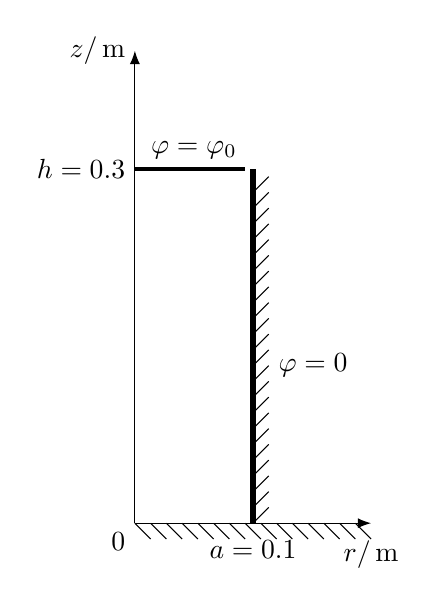
\begin{tikzpicture}
		\draw [-Latex] (0,0) -- (3,0);
		\node [below] at (3,-0.1) {$r/\m$};
		\draw [-Latex] (0,0) -- (0,6);
		\node [left] at (0,6) {$z/\m$};
		\node [below left] at (0,0) {$0$}; 
		
		\draw [line width = 2pt] (1.5,0) -- (1.5,4.5);
		\node [below] at (1.5,-0.1) {$a=0.1$};
		\draw [line width = 1.5pt] (0,4.5) -- (1.4,4.5);
		\node [left] at (0,4.5) {$h=0.3$};
		
		\foreach \x in {0,0.2,...,4.3}
			\draw (1.5,\x) -- (1.7,\x +0.2);
		\foreach \x in {0,0.2,...,2.8}
			\draw (\x,0) -- (\x+0.2,-0.2);
		
		\node [right] at (1.7,2) {$\varphi = 0$};
		\node [above] at (0.75,4.5) {$\varphi = \varphi_0$};
	\end{tikzpicture}
\end{figure}

\begin{figure}
	\centering
	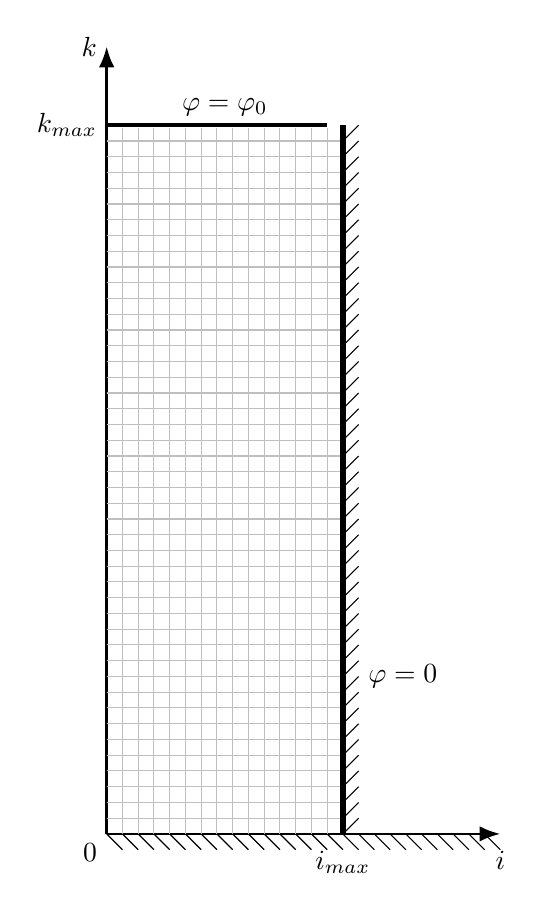
\begin{tikzpicture}
	\draw [-Latex, line width = 1pt] (0,0) -- (5,0);
	\node [below] at (5,-0.1) {$i$};
	\draw [-Latex, line width = 1pt] (0,0) -- (0,10);
	\node [left] at (0,10) {$k$};
	\node [below left] at (0,0) {$0$}; 
	
	\draw [line width = 2pt] (3,0) -- (3,9);
	\node [below] at (3,-0.1) {$i_{max}$};
	\draw [line width = 1.5pt] (0,9) -- (2.8,9);
	\node [left] at (0,9) {$k_{max}$};
	
	\foreach \x in {0,0.2,...,8.8}
		\draw (3,\x) -- (3.2,\x +0.2);
	\foreach \x in {0,0.2,...,4.8}
		\draw (\x,0) -- (\x+0.2,-0.2);
	
	\node [right] at (3.2,2) {$\varphi = 0$};
	\node [above] at (1.5,9) {$\varphi = \varphi_0$};
	
	\foreach \x in {0.2,0.4,...,2.8}
		\draw [gray!50] (\x,0) -- (\x,8.97);
	\foreach \x in {0.2,0.4,...,8.8}
		\draw [gray!50] (0,\x) -- (2.965,\x);
	\end{tikzpicture}
\end{figure}

\begin{figure}
	\centering
	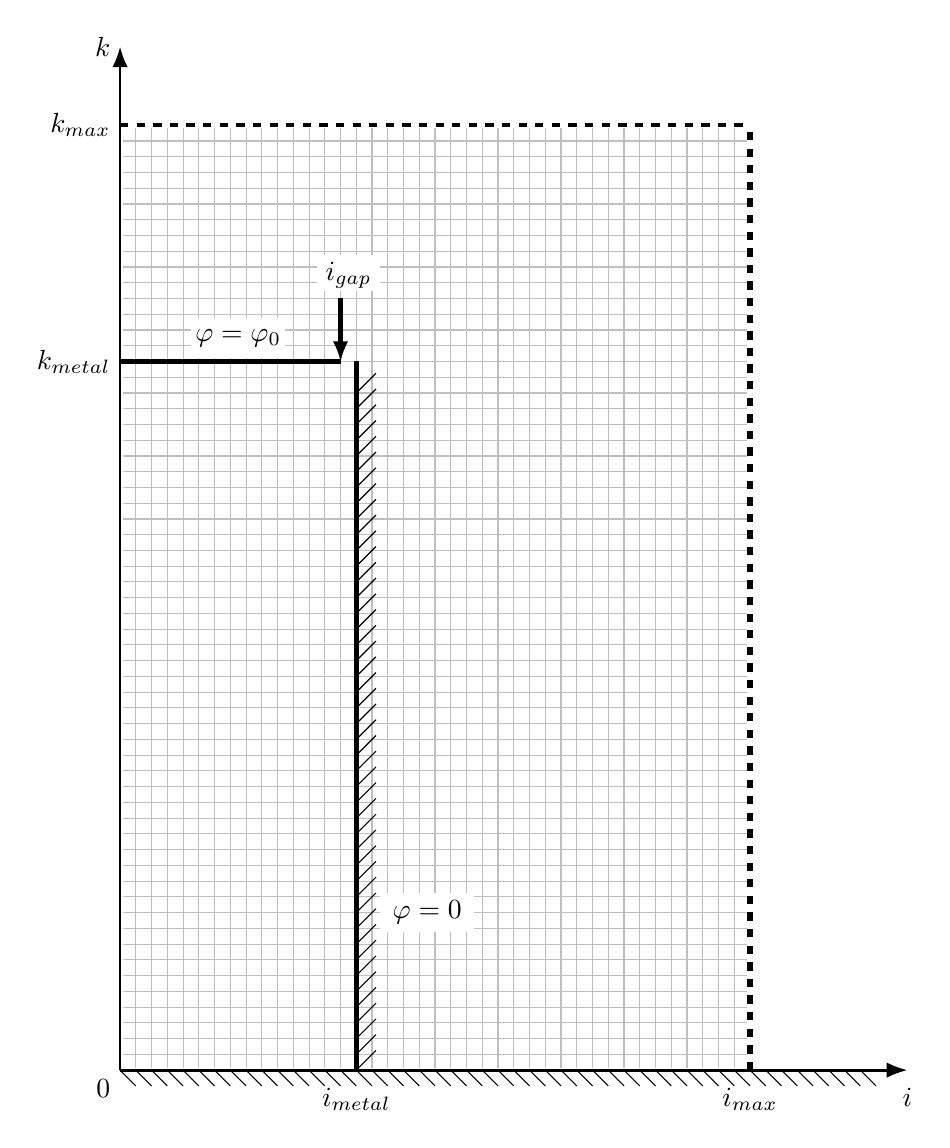
\begin{tikzpicture}
	\foreach \x in {0.2,0.4,...,7.8}
		\draw [gray!50] (\x,0.03) -- (\x,11.97);
	\foreach \x in {0.2,0.4,...,11.8}
		\draw [gray!50] (0.035,\x) -- (7.965,\x);
	
	\draw [-Latex, line width = 1pt] (0,0) -- (10,0);
	\node [below] at (10,-0.1) {$i$};
	\draw [-Latex, line width = 1pt] (0,0) -- (0,13);
	\node [left] at (0,13) {$k$};
	\node [below left] at (0,0) {$0$}; 
	
	\draw [line width = 2pt] (3,0) -- (3,9);
	\node [below] at (3,-0.1) {$i_{metal}$};
	\draw [line width = 1.5pt] (0,9) -- (2.8,9);
	\node [left] at (0,9) {$k_{metal}$};
	
	\draw [dashed,line width = 2pt] (8,0) -- (8,12);
	\node [below] at (8,-0.1) {$i_{max}$};
	\draw [dashed,line width = 1.5pt] (0,12) -- (8,12);
	\node [left] at (0,12) {$k_{max}$};
	
	\foreach \x in {0,0.2,...,8.75}
	\draw (3,\x) -- (3.25,\x +0.25);
	\foreach \x in {0,0.2,...,9.4}
	\draw (\x,0) -- (\x+0.2,-0.2);
	
	\fill [white] (3.9-0.6,2-0.25) rectangle (3.9+0.6,2+0.25);
	\node  at (3.9,2) {$\varphi = 0$};
	\fill [white] (1.5-0.6,9.3-0.25) rectangle (1.5+0.6,9.3+0.25);
	\node at (1.5,9.3) {$\varphi = \varphi_0$};
	
	\draw [-latex,line width = 1.5pt] (2.8,9.8) -- (2.8,9);
	\fill [white] (2.9-0.4,10.1-0.2) rectangle (2.9+0.4,10.1+0.25);
	\node [above] at (2.9,9.8) {$i_{gap}$};
	
	\end{tikzpicture}
\end{figure}
	
	
\begin{figure}
	\centering
	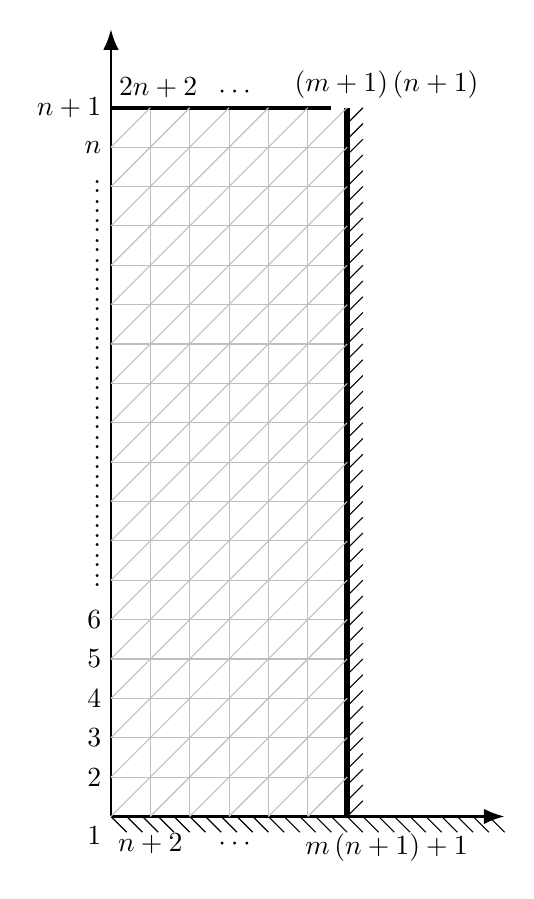
\begin{tikzpicture}
	\draw [-Latex, line width = 1pt] (0,0) -- (5,0);
	
	\draw [-Latex, line width = 1pt] (0,0) -- (0,10);
	
	\node [below left] at (0,0) {$1$}; 
	
	\draw [line width = 2pt] (3,0) -- (3,9);
	\node [below] at (3.5,-0.1) {$m\left(n+1\right)+1$};
	\draw [line width = 1.5pt] (0,9) -- (2.8,9);
	\node [left] at (0,9) {$n+1$};
	\node [above] at (3.5,9) {$\left(m+1\right)\left(n+1\right)$};
	
	\foreach \x in {0,0.2,...,8.8}
	\draw (3,\x) -- (3.2,\x +0.2);
	\foreach \x in {0,0.2,...,4.8}
	\draw (\x,0) -- (\x+0.2,-0.2);

	
	\foreach \x in {0.5,1,...,2.5}
	\draw [gray!50] (\x,0) -- (\x,8.97);
	\foreach \x in {0.5,1,...,8.5}
	\draw [gray!50] (0,\x) -- (2.965,\x);
	\node [left] at (0,0.5) {$2$};
	\node [left] at (0,1) {$3$};
	\node [left] at (0,1.5) {$4$};
	\node [left] at (0,2) {$5$};
	\node [left] at (0,2.5) {$6$};
	\foreach \x in {3,3.25,...,8}
		\node [left] at (0,\x) {:};
	\node [left] at (0,8.5) {$n$};	
	\node [below] at (0.5,-0.1) {$n+2$};
	\node [above] at (0.6,9) {$2n+2$};
	\node [below] at (1.6,-0.15) {$\cdots$};
	\node [above] at (1.6,9) {$\cdots$};
	
	\foreach \x in {0,0.5,...,2.5}
		\foreach \y in {0,0.5,...,8.5}
			\draw [gray!50] (\x,\y) -- (\x+0.5,\y+0.5); 
	\end{tikzpicture}
\end{figure}
	
	
	
\end{document}